%%%%%%%%%%%%%%%%%%%%%%%%%%%%%%%%%%%%
% Lesson Plan (50 minutes)
%%%%%%%%%%%%%%%%%%%%%%%%%%%%%%%%%%%%
\begin{frame}
    \frametitle{Lesson Plan}
    \begin{itemize}
        \item xx min Lecture: Normal distribution (cont.), 68-95-99.7, describing variability
        \item xx min R Demonstration: 68-95-99.7 rule examples (more on variability)
        \item xx min Edfinity quiz: Variability
        \item xx min Lecture: review quiz answers
    \end{itemize}
\end{frame}

%%%%%%%%%%%%%%%%%%%%%%%%%%%%%%%%%%%%
% Learning objectives:
%%%%%%%%%%%%%%%%%%%%%%%%%%%%%%%%%%%%
\begin{frame}
    \frametitle{Learning Objectives}
    \begin{itemize}
        \item \textbf{M1 LO3: Use R for Data Management and Exploration:} Utilize R to load, pre-process, and explore data through visualization and summarization techniques.
        \item \textbf{M6 LO1: Validate and Explain Probability Distributions:} Assess the validity of a probability distribution using the concepts of outcome, sample space, and probability properties (e.g., disjoint outcomes, probabilities between 0 and 1, and total probabilities summing to 1).
        \item \textbf{M6 LO3: Compute Probabilities Using Various Tools:} Use logic, Venn diagrams, and probability rules to compute probabilities for events.
        \item \textbf{M6 LO4: Understand and Compute Expectations and Variances:} Explain the concepts of expectations and variances of random variables, and compute the expectation and variance of a linear combination of random variables.
        \item \textbf{M6 LO6: Assess Data Using the Normal Distribution:} Use the normal distribution to assess the "unusualness" of data points, apply the 68-95-99.7% rule, evaluate normality through histograms and q-q plots, and determine when a normal approximation to the binomial model is valid for calculating binomial probabilities.
    \end{itemize}
\end{frame}

%%%%%%%%%%%%%%%%%%%%%%%%%%%%%%%%%%%%
% TODO: Copy and adapt these slides base on the lesson plan
%%%%%%%%%%%%%%%%%%%%%%%%%%%%%%%%%%%%

\section{Normal distribution}

%%%%%%%%%%%%%%%%%%%%%%%%%%%%%%%%%%%%

\begin{frame}
\frametitle{Normal distribution}

\begin{itemize}

\item Unimodal and symmetric, bell shaped curve

\item Many variables are nearly normal, but none are exactly normal

\item Denoted as \mathhl{N(\mu,\sigma)} $\rightarrow$ Normal with mean $\mu$ and standard deviation $\sigma$

\end{itemize}

\begin{center}
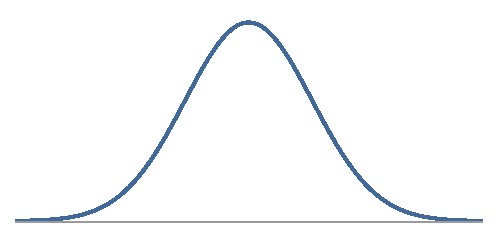
\includegraphics[width=0.7\textwidth]{4-1_normal_distribution/figures/simpleNormal/simpleNormal}
\end{center}

\end{frame}

%%%%%%%%%%%%%%%%%%%%%%%%%%%%%%%%%%%%

\begin{frame}
\frametitle{Heights of males}

\twocol{0.5}{0.5}{
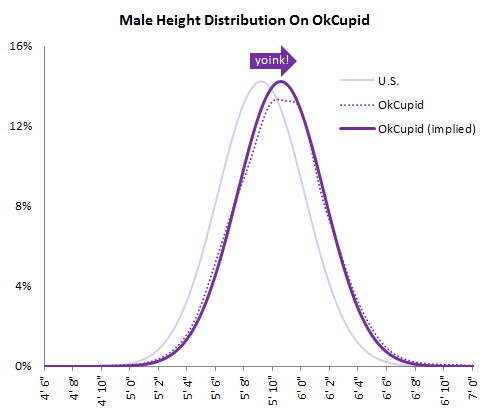
\includegraphics[width=\textwidth]{4-1_normal_distribution/figures/ok_cupid/ok_cupid_men} \\
}
{
\pause
{\footnotesize``The male heights on OkCupid very nearly follow the expected normal distribution -- except the whole thing is shifted to the right of where it should be. Almost universally guys like to add a couple inches." 

``You can also see a more subtle vanity at work: starting at roughly 5' 8", the top of the dotted curve tilts even further rightward. This means that guys as they get closer to six feet round up a bit more than usual, stretching for that coveted psychological benchmark."
}
}

\ct{\webURL{http://blog.okcupid.com/index.php/the-biggest-lies-in-online-dating/}}

\end{frame}

%%%%%%%%%%%%%%%%%%%%%%%%%%%%%%%%%%%%

\begin{frame}
\frametitle{Heights of females}

\twocol{0.5}{0.5}{
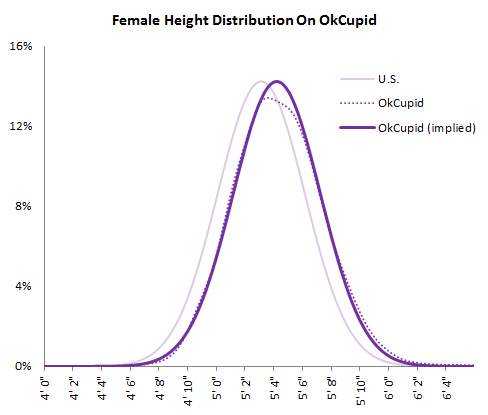
\includegraphics[width=\textwidth]{4-1_normal_distribution/figures/ok_cupid/ok_cupid_women} \\
}
{
\pause
{\footnotesize ``When we looked into the data for women, we were surprised to see height exaggeration was just as widespread, though without the lurch towards a benchmark height."
}
}

\vfill

\ct{\webURL{http://blog.okcupid.com/index.php/the-biggest-lies-in-online-dating/}}

\end{frame}

%%%%%%%%%%%%%%%%%%%%%%%%%%%%%%%%%%%%

\subsection{Normal distribution model}

%%%%%%%%%%%%%%%%%%%%%%%%%%%%%%%%%%%%

\begin{frame}
\frametitle{Normal distributions with different parameters}

\vspace{-0.5cm}
\begin{center}
$\mu$: mean, $\sigma$: standard deviation
\[N(\mu = 0, \sigma = 1) \hspace{1.4cm} N(\mu = 19, \sigma = 4) \]
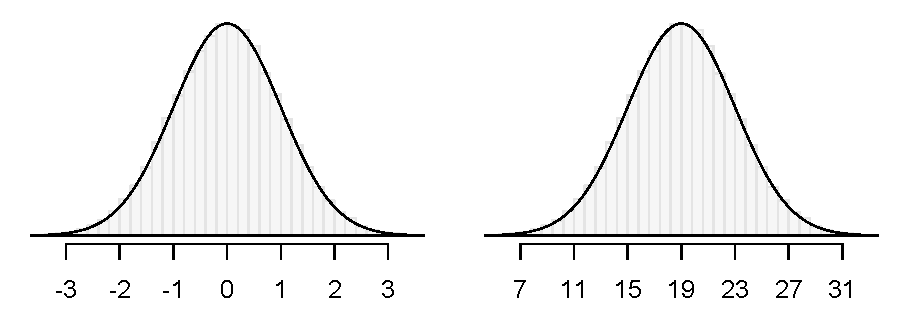
\includegraphics[width=0.6\textwidth]{4-1_normal_distribution/figures/twoSampleNormals/twoSampleNormals} \\
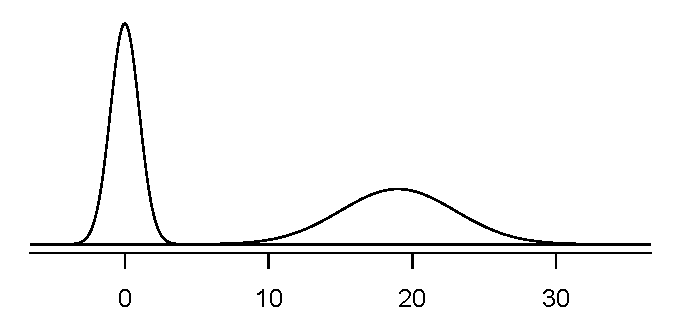
\includegraphics[width=0.6\textwidth]{4-1_normal_distribution/figures/twoSampleNormalsStacked/twoSampleNormalsStacked}
\end{center}

\end{frame}

%%%%%%%%%%%%%%%%%%%%%%%%%%%%%%%%%%%%

\subsection{Standardizing with Z scores}

%%%%%%%%%%%%%%%%%%%%%%%%%%%%%%%%%%%%

\begin{frame}
\frametitle{}

\dq{SAT scores are distributed nearly normally with mean 1500 and standard deviation 300. ACT scores are distributed nearly normally with mean 21 and standard deviation 5. A college admissions officer wants to determine which of the two applicants scored better on their standardized test with respect to the other test takers: Pam, who earned an 1800 on her SAT, or Jim, who scored a 24 on his ACT?}

\begin{center}
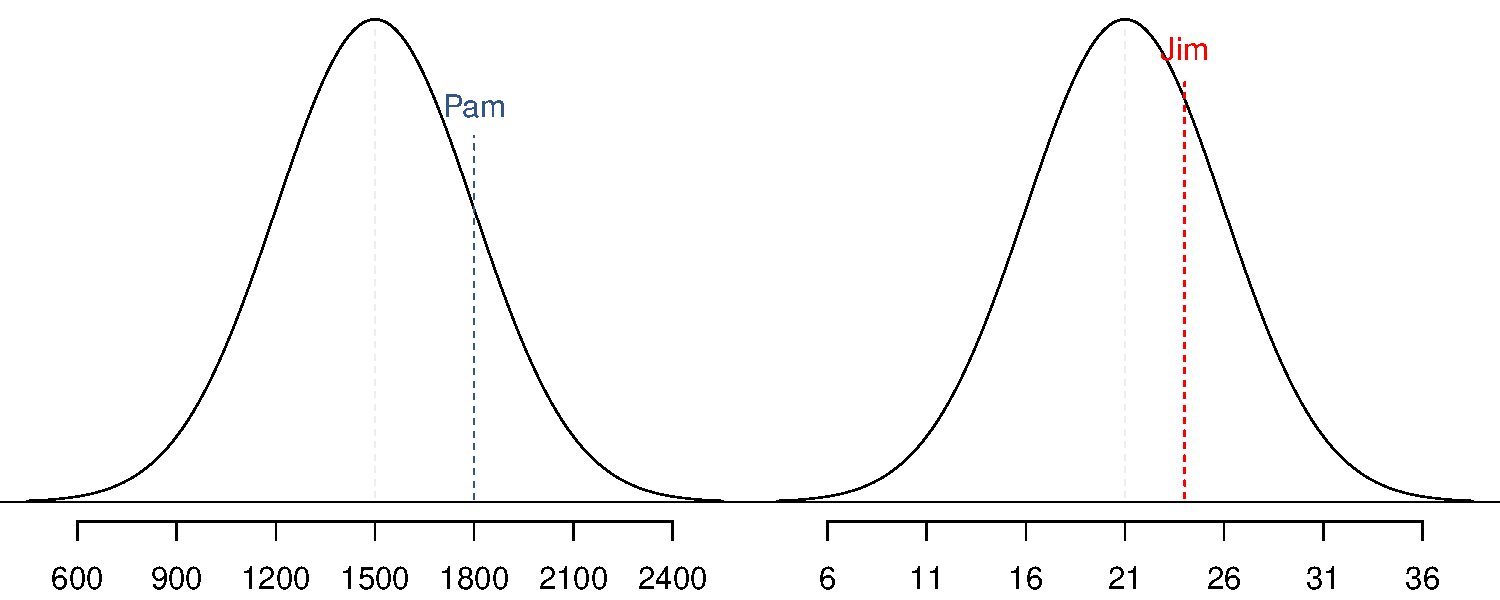
\includegraphics[width=\textwidth]{4-1_normal_distribution/figures/satActNormals/satActNormals}
\end{center}

\end{frame}

%%%%%%%%%%%%%%%%%%%%%%%%%%%%%%%%%%%%

\begin{frame}
\frametitle{Standardizing with Z scores}

Since we cannot just compare these two raw scores, we instead compare how many standard deviations beyond the mean each observation is.

\begin{itemize}

\item Pam's score is $\frac{1800 - 1500}{300} = 1$ standard deviation above the mean.

\item Jim's score is $\frac{24 - 21}{5} = 0.6$ standard deviations above the mean.

\end{itemize}

\begin{center}
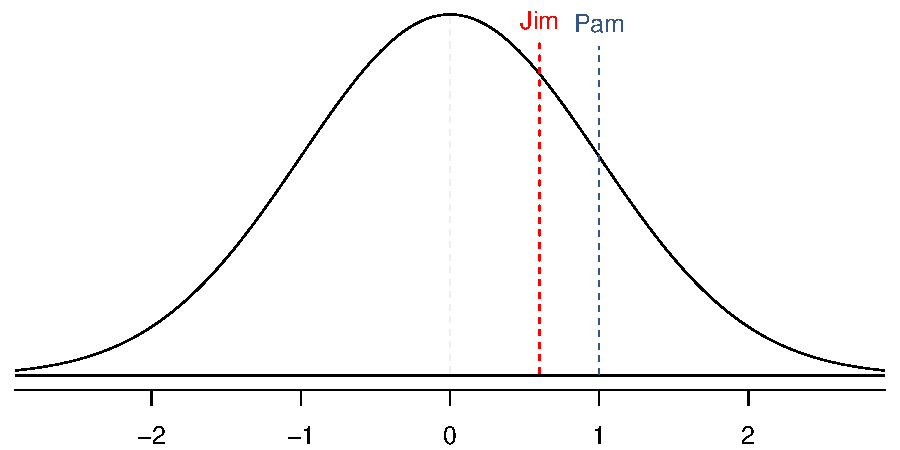
\includegraphics[width=0.7\textwidth]{4-1_normal_distribution/figures/satActNormals/satActNormalsStandardized}
\end{center}

\end{frame}

%%%%%%%%%%%%%%%%%%%%%%%%%%%%%%%%%%%%

\begin{frame}
\frametitle{Standardizing with Z scores (cont.)}

\begin{itemize}

\item These are called \hl{standardized} scores, or \hl{Z scores}.

\item Z score of an observation is the number of standard deviations it falls above or below the mean.
\formula{\[Z = \frac{observation - mean}{SD}\]}

\item Z scores are defined for distributions of any shape, but only when the distribution is normal can we use Z scores to calculate percentiles.

\item Observations that are more than 2 SD away from the mean ($|Z| > 2$) are usually considered unusual.

\end{itemize}

\end{frame}

%%%%%%%%%%%%%%%%%%%%%%%%%%%%%%%%%%%%

\begin{frame}
\frametitle{Percentiles}

\begin{itemize}

\item \hl{Percentile} is the percentage of observations that fall below a given data point. 

\item Graphically, percentile is the area below the probability distribution curve to the left of that observation.

\end{itemize}

\begin{center}
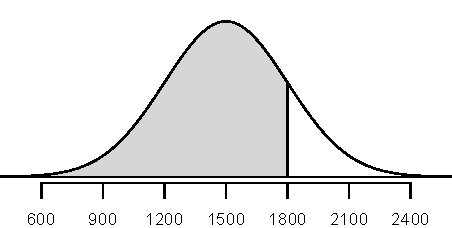
\includegraphics[width=0.7\textwidth]{4-1_normal_distribution/figures/satBelow1800/satBelow1800}
\end{center}

\end{frame}

%%%%%%%%%%%%%%%%%%%%%%%%%%%%%%%%%%%%

%\begin{frame}
%\frametitle{}
%
%\dq{Approximately what percent of students score below 1800 on the SAT? (Hint: Use the 68-95-99.7\% rule.)}
%
%\only<1>{
%\begin{center}
%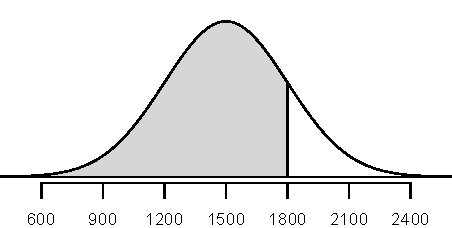
\includegraphics[width=0.7\textwidth]{4-1_normal_distribution/figures/satBelow1800/satBelow1800}
%\end{center}
%}
%
%\only<2 | handout:0>{
%\begin{center}
%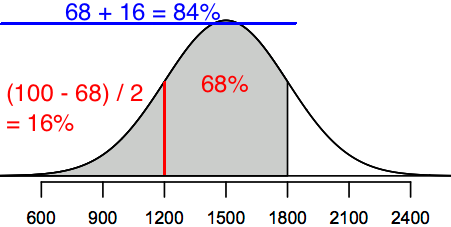
\includegraphics[width=0.7\textwidth]{4-1_normal_distribution/figures/satBelow1800/satBelow1800_soln}
%\end{center}
%}
%
%\soln{\only<2>{
%\begin{align*}
%100 - 68 &= 32\% \\
%32 / 2 &= 16\% \\
%68 + 16 &= 84\%
%\end{align*}}}
%
%\end{frame}
%
%%%%%%%%%%%%%%%%%%%%%%%%%%%%%%%%%%%%%

\subsection{Finding tail areas}

%%%%%%%%%%%%%%%%%%%%%%%%%%%%%%%%%%%%

\begin{frame}[fragile]
\frametitle{Calculating percentiles - using computation}

There are many ways to compute percentiles/areas under the curve:

\begin{itemize}
\item R:
\end{itemize}
\begin{beamerboxesrounded}[shadow = false, lower = code body]{}
{\small \begin{verbatim}
> pnorm(1800, mean = 1500, sd = 300)
[1] 0.8413447
\end{verbatim}
}
\end{beamerboxesrounded}
\begin{itemize}
\item Applet: {\small \webURL{https://gallery.shinyapps.io/dist_calc/}}
\begin{center}
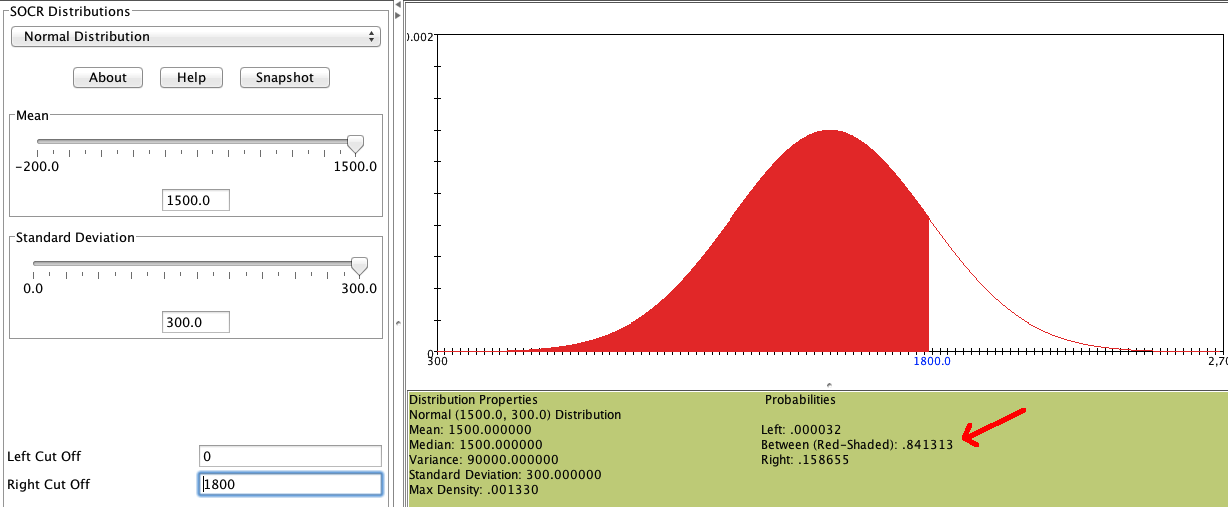
\includegraphics[width=0.8\textwidth]{4-1_normal_distribution/figures/applet}
\end{center}

\end{itemize}


\end{frame}

%%%%%%%%%%%%%%%%%%%%%%%%%%%%%%%%%%%%

\begin{frame}[fragile]
\frametitle{Calculating percentiles - using tables}

{\footnotesize
\begin{tabular}{c | >{\columncolor[gray]{0.6}[0pt]}rrrrr | rrrrr |}
  \cline{2-11}
&&&& \multicolumn{4}{c}{Second decimal place of $Z$} &&& \\
  \cline{2-11}
$Z$ & 0.00 & 0.01 & 0.02 & 0.03 & 0.04 & 0.05 & 0.06 & 0.07 & 0.08 & 0.09 \\
  \hline
  \hline
0.0 & \tiny{0.5000} & \tiny{0.5040} & \tiny{0.5080} & \tiny{0.5120} & \tiny{0.5160} & \tiny{0.5199} & \tiny{0.5239} & \tiny{0.5279} & \tiny{0.5319} & \tiny{0.5359} \\
  0.1 & \tiny{0.5398} & \tiny{0.5438} & \tiny{0.5478} & \tiny{0.5517} & \tiny{0.5557} & \tiny{0.5596} & \tiny{0.5636} & \tiny{0.5675} & \tiny{0.5714} & \tiny{0.5753} \\
  0.2 & \tiny{0.5793} & \tiny{0.5832} & \tiny{0.5871} & \tiny{0.5910} & \tiny{0.5948} & \tiny{0.5987} & \tiny{0.6026} & \tiny{0.6064} & \tiny{0.6103} & \tiny{0.6141} \\
  0.3 & \tiny{0.6179} & \tiny{0.6217} & \tiny{0.6255} & \tiny{0.6293} & \tiny{0.6331} & \tiny{0.6368} & \tiny{0.6406} & \tiny{0.6443} & \tiny{0.6480} & \tiny{0.6517} \\
  0.4 & \tiny{0.6554} & \tiny{0.6591} & \tiny{0.6628} & \tiny{0.6664} & \tiny{0.6700} & \tiny{0.6736} & \tiny{0.6772} & \tiny{0.6808} & \tiny{0.6844} & \tiny{0.6879} \\
  \hline
  0.5 & \tiny{0.6915} & \tiny{0.6950} & \tiny{0.6985} & \tiny{0.7019} & \tiny{0.7054} & \tiny{0.7088} & \tiny{0.7123} & \tiny{0.7157} & \tiny{0.7190} & \tiny{0.7224} \\
  0.6 & \tiny{0.7257} & \tiny{0.7291} & \tiny{0.7324} & \tiny{0.7357} & \tiny{0.7389} & \tiny{0.7422} & \tiny{0.7454} & \tiny{0.7486} & \tiny{0.7517} & \tiny{0.7549} \\
  0.7 & \tiny{0.7580} & \tiny{0.7611} & \tiny{0.7642} & \tiny{0.7673} & \tiny{0.7704} & \tiny{0.7734} & \tiny{0.7764} & \tiny{0.7794} & \tiny{0.7823} & \tiny{0.7852} \\
  0.8 & \tiny{0.7881} & \tiny{0.7910} & \tiny{0.7939} & \tiny{0.7967} & \tiny{0.7995} & \tiny{0.8023} & \tiny{0.8051} & \tiny{0.8078} & \tiny{0.8106} & \tiny{0.8133} \\
  0.9 & \tiny{0.8159} & \tiny{0.8186} & \tiny{0.8212} & \tiny{0.8238} & \tiny{0.8264} & \tiny{0.8289} & \tiny{0.8315} & \tiny{0.8340} & \tiny{0.8365} & \tiny{0.8389} \\
  \hline
  \hline
\rowcolor[gray]{.6}
  1.0 & \orange{\tiny{0.8413}} & \tiny{0.8438} & \tiny{0.8461} & \tiny{0.8485} & \tiny{0.8508} & \tiny{0.8531} & \tiny{0.8554} & \tiny{0.8577} & \tiny{0.8599} & \tiny{0.8621} \\
  1.1 & \tiny{0.8643} & \tiny{0.8665} & \tiny{0.8686} & \tiny{0.8708} & \tiny{0.8729} & \tiny{0.8749} & \tiny{0.8770} & \tiny{0.8790} & \tiny{0.8810} & \tiny{0.8830} \\
  1.2 & \tiny{0.8849} & \tiny{0.8869} & \tiny{0.8888} & \tiny{0.8907} & \tiny{0.8925} & \tiny{0.8944} & \tiny{0.8962} & \tiny{0.8980} & \tiny{0.8997} & \tiny{0.9015} \\
\end{tabular}
}

\end{frame}

%%%%%%%%%%%%%%%%%%%%%%%%%%%%%%%%%%%%

\subsection{Normal probability examples}

%%%%%%%%%%%%%%%%%%%%%%%%%%%%%%%%%%%%

\begin{frame}
\frametitle{Six sigma}

``The term \textit{six sigma process} comes from the notion that if one has six standard deviations between the process mean and the nearest specification limit, as shown in the graph, practically no items will fail to meet specifications."

\begin{center}

\includegraphics[width=0.35\textwidth]{4-1_normal_distribution/figures/sixsigma}
\end{center}

\ct{\webURL{http://en.wikipedia.org/wiki/Six_Sigma}}

\end{frame}

%%%%%%%%%%%%%%%%%%%%%%%%%%%%%%%%%%%%

\begin{frame}
\frametitle{Quality control}

\dq{{\small At Heinz ketchup factory the amounts which go into bottles of ketchup are supposed to be normally distributed with mean 36 oz. and standard deviation 0.11 oz. Once every 30 minutes a bottle is selected from the production line, and its contents are noted precisely. If the amount of ketchup in the bottle is below 35.8 oz. or above 36.2 oz., then the bottle fails the quality control inspection. What percent of bottles have less than 35.8 ounces of ketchup?}}

\soln{\pause
Let $X$ = amount of ketchup in a bottle: $X \sim N(\mu = 36, \sigma = 0.11)$ \\
\pause
\twocol{0.4}{0.6}{
\begin{center}
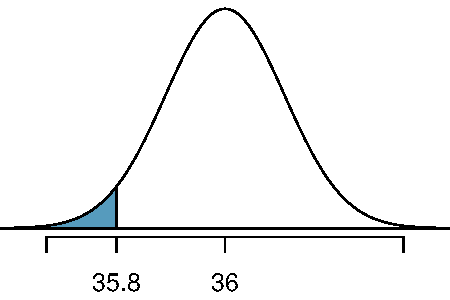
\includegraphics[width=\textwidth]{4-1_normal_distribution/figures/ketchup/ketchupLT358}
\end{center}
}
{
\pause
\[ Z = \frac{35.8 - 36}{0.11} = -1.82 \]
}
}

\end{frame}

%%%%%%%%%%%%%%%%%%%%%%%%%%%%%%%%%%%%

\begin{frame}[fragile]
\frametitle{Finding the exact probability - using R}

\begin{beamerboxesrounded}[shadow = true, lower = code body]{}
{\small \begin{verbatim}
> pnorm(-1.82, mean = 0, sd = 1)
[1] 0.0344
\end{verbatim}
}
\end{beamerboxesrounded}

$\:$ \\
\pause

OR

$\:$ \\
\pause

\begin{beamerboxesrounded}[shadow = true, lower = code body]{}
{\small \begin{verbatim}
> pnorm(35.8, mean = 36, sd = 0.11)
[1] 0.0345
\end{verbatim}
}
\end{beamerboxesrounded}


\end{frame}

%%%%%%%%%%%%%%%%%%%%%%%%%%%%%%%%%%%%%

\begin{frame}
\frametitle{Practice}

\pq{What percent of bottles \underline{pass} the quality control inspection?}

\vspace{-0.5cm}
\begin{multicols}{2}
\begin{enumerate}[(a)]
\item 1.82\%
\item 3.44\%
\item 6.88\%
\solnMult{93.12\%}
\item 96.56\%
\item[]
\end{enumerate}
\end{multicols}

\soln{
\vspace{-0.5cm}
\pause
\begin{columns}[c]
\column{0.3\textwidth}
\pause
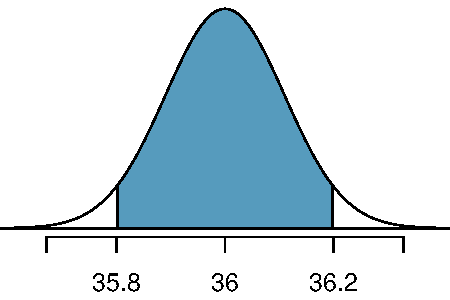
\includegraphics[width=\textwidth]{4-1_normal_distribution/figures/ketchup/ketchupBET}
\column{0.05\textwidth}
=
\pause
\column{0.3\textwidth}
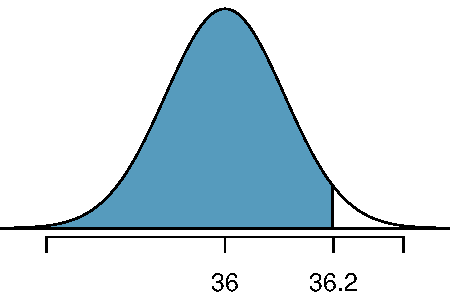
\includegraphics[width=\textwidth]{4-1_normal_distribution/figures/ketchup/ketchupLT362}
\column{0.05\textwidth}
-
\pause
\column{0.3\textwidth}
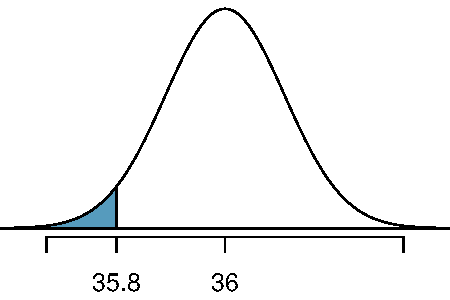
\includegraphics[width=\textwidth]{4-1_normal_distribution/figures/ketchup/ketchupLT358}
\end{columns}
\pause
\begin{eqnarray*}
Z_{35.8} &=& \frac{35.8 - 36}{0.11} = -1.82 \\ \pause
Z_{36.2} &=& \frac{36.2 - 36}{0.11} = 1.82 \\ \pause
P(35.8 < X < 36.2) &=& P(-1.82 < Z < 1.82) = 0.9656 - 0.0344 = 0.9312
\end{eqnarray*}
}

\end{frame}

%%%%%%%%%%%%%%%%%%%%%%%%%%%%%%%%%%%%

\begin{frame}[fragile]
\frametitle{Finding cutoff points}

\dq{Body temperatures of healthy humans are distributed nearly normally with mean 98.2$\degree$F and standard deviation 0.73$\degree$F. What is the cutoff for the lowest 3\% of human body temperatures?}

\pause

\twocol{0.3}{0.7}
{
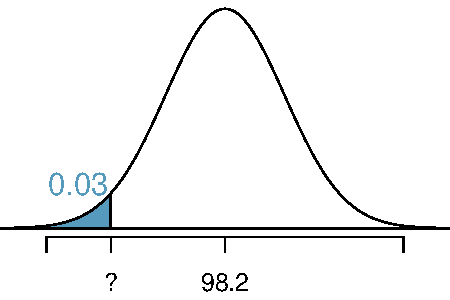
\includegraphics[width=\textwidth]{4-1_normal_distribution/figures/temp/tempLOW3PERC}
}
{
\pause
\begin{eqnarray*}
P(X < x) &=& 0.03 \rightarrow P(Z < \orange{-1.88}) = 0.03 \\ \pause
Z &=& \frac{obs~-~mean}{SD} \rightarrow \frac{x - 98.2}{0.73} = -1.88 \\ \pause
x &=& (-1.88 \times 0.73) + 98.2 = 96.8\degree F
\end{eqnarray*}
}
$\:$ \\
\begin{beamerboxesrounded}[shadow = true, lower = code body]{}
{\small \begin{verbatim}
> qnorm(0.03)
[1] -1.880794
\end{verbatim}
}
\end{beamerboxesrounded}

\ct{Mackowiak, Wasserman, and Levine (1992), \textit{A Critical Appraisal of 98.6 Degrees F, the Upper Limit of the Normal Body Temperature, and Other Legacies of Carl Reinhold August Wunderlick}.}

\end{frame}

%%%%%%%%%%%%%%%%%%%%%%%%%%%%%%%%%%%

\begin{frame}[fragile]
\frametitle{Practice}

\pq{Body temperatures of healthy humans are distributed nearly normally with mean 98.2$\degree$F and standard deviation 0.73$\degree$F. What is the cutoff for the highest 10\% of human body temperatures?}

\vspace{-0.5cm}
\begin{multicols}{2}
\begin{enumerate}[(a)]
\item 97.3$\degree$F
\solnMult{99.1$\degree$F}
\item 99.4$\degree$F
\item 99.6$\degree$F
\end{enumerate}
\end{multicols}

\soln{
\vspace{-0.5cm}
\pause
\twocol{0.3}{0.7}
{
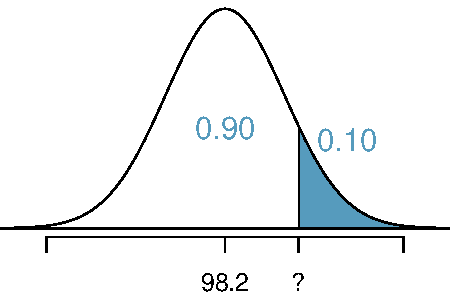
\includegraphics[width=\textwidth]{4-1_normal_distribution/figures/temp/tempHIGH10PERC}
}
{
\pause
\begin{eqnarray*}
P(X > x) &=& 0.10 \rightarrow P(Z < \orange{1.28}) = 0.90 \\ \pause
Z &=& \frac{obs~-~mean}{SD} \rightarrow \frac{x - 98.2}{0.73} = 1.28 \\ \pause
x &=& (1.28 \times 0.73) + 98.2 = 99.1
\end{eqnarray*}
}
}

\end{frame}

%%%%%%%%%%%%%%%%%%%%%%%%%%%%%%%%%%%

\subsection{68-95-99.7 rule}

%%%%%%%%%%%%%%%%%%%%%%%%%%%%%%%%%%%%

\begin{frame}
\frametitle{68-95-99.7 Rule}

\begin{itemize}

\item For nearly normally distributed data, 
\begin{itemize}
\item about 68\% falls within 1 SD of the mean,
\item about 95\% falls within 2 SD of the mean,
\item about 99.7\% falls within 3 SD of the mean.
\end{itemize}

\item It is possible for observations to fall 4, 5, or more standard deviations away from the mean, but these occurrences are very rare if the data are nearly normal.

\end{itemize}

\begin{center}
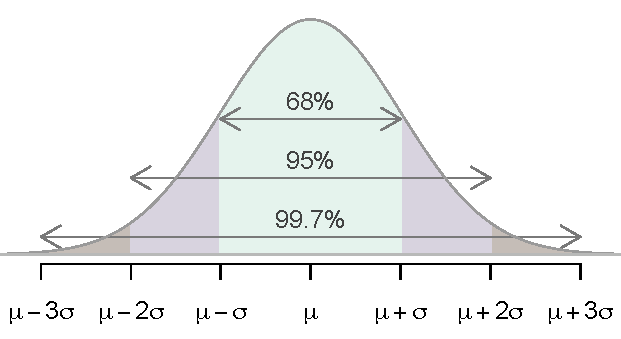
\includegraphics[width=0.7\textwidth]{4-1_normal_distribution/figures/6895997/6895997}
\end{center}

\end{frame}

%%%%%%%%%%%%%%%%%%%%%%%%%%%%%%%%%%%%

\begin{frame}
\frametitle{Describing variability using the 68-95-99.7 Rule}

SAT scores are distributed nearly normally with mean 1500 and standard deviation 300.

\pause
\begin{itemize}

\item $\sim$68\% of students score between 1200 and 1800 on the SAT. 

\item $\sim$95\% of students score between 900 and 2100 on the SAT. 

\item $\sim$99.7\% of students score between 600 and 2400 on the SAT. 

\end{itemize}

\begin{center}
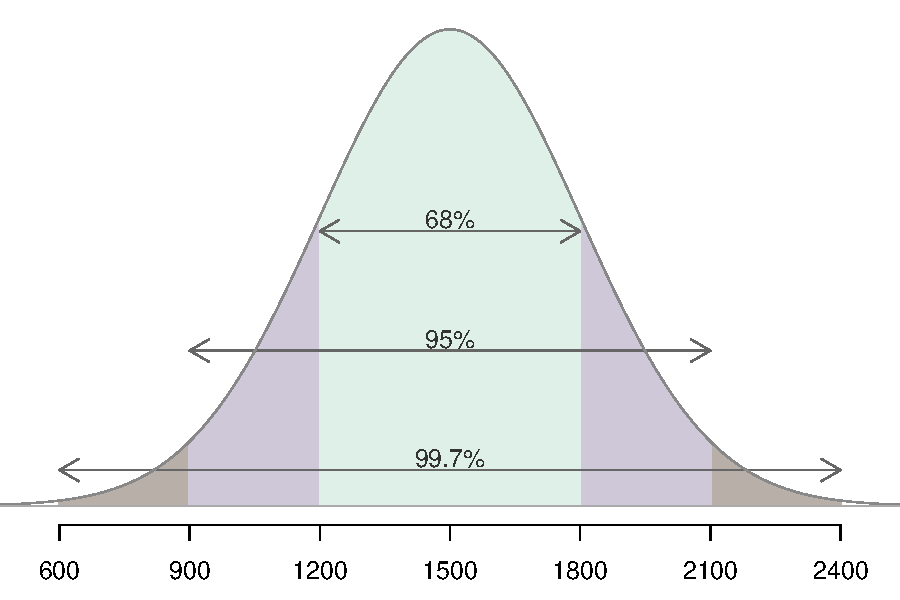
\includegraphics[width=0.65\textwidth]{4-1_normal_distribution/figures/sat_empirical/sat_empirical}
\end{center}

\end{frame}

%%%%%%%%%%%%%%%%%%%%%%%%%%%%%%%%%%%%

\begin{frame}[fragile]
\frametitle{Number of hours of sleep on school nights}

\only<1 | handout:0>{
\begin{center}
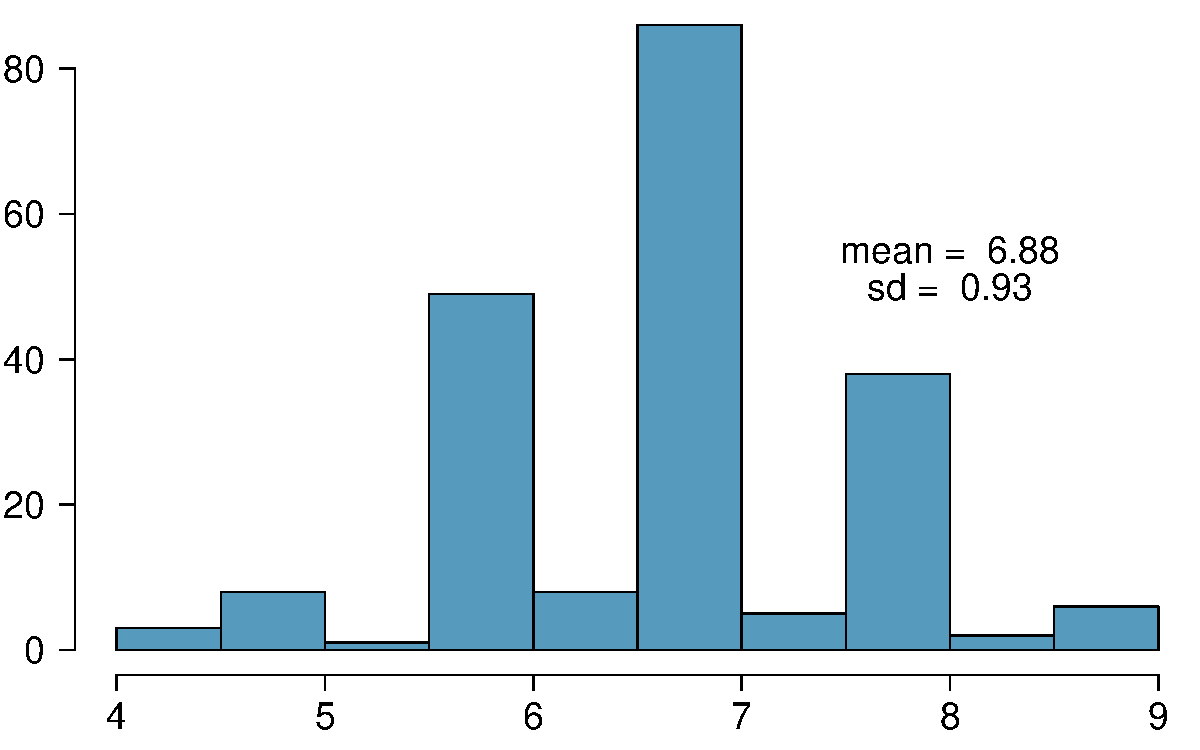
\includegraphics[width=0.75\textwidth]{4-1_normal_distribution/figures/sleep/sleep-hist} 
\end{center}
\vspace{-0.25cm}
\begin{itemize}
\item Mean = 6.88 hours, SD = 0.92 hrs
\item[] \textcolor{white}{72\% of the data are within 1 SD of the mean: $6.88 \pm 0.93$}
\item[] \textcolor{white}{92\% of the data are within 2 SD of the mean: $6.88 \pm 2 \times 0.93$}
\item[] \textcolor{white}{99\% of the data are within 3 SD of the mean: $6.88 \pm 3 \times 0.93$}
\end{itemize}
}

\only<2 | handout:0>{
\begin{center}
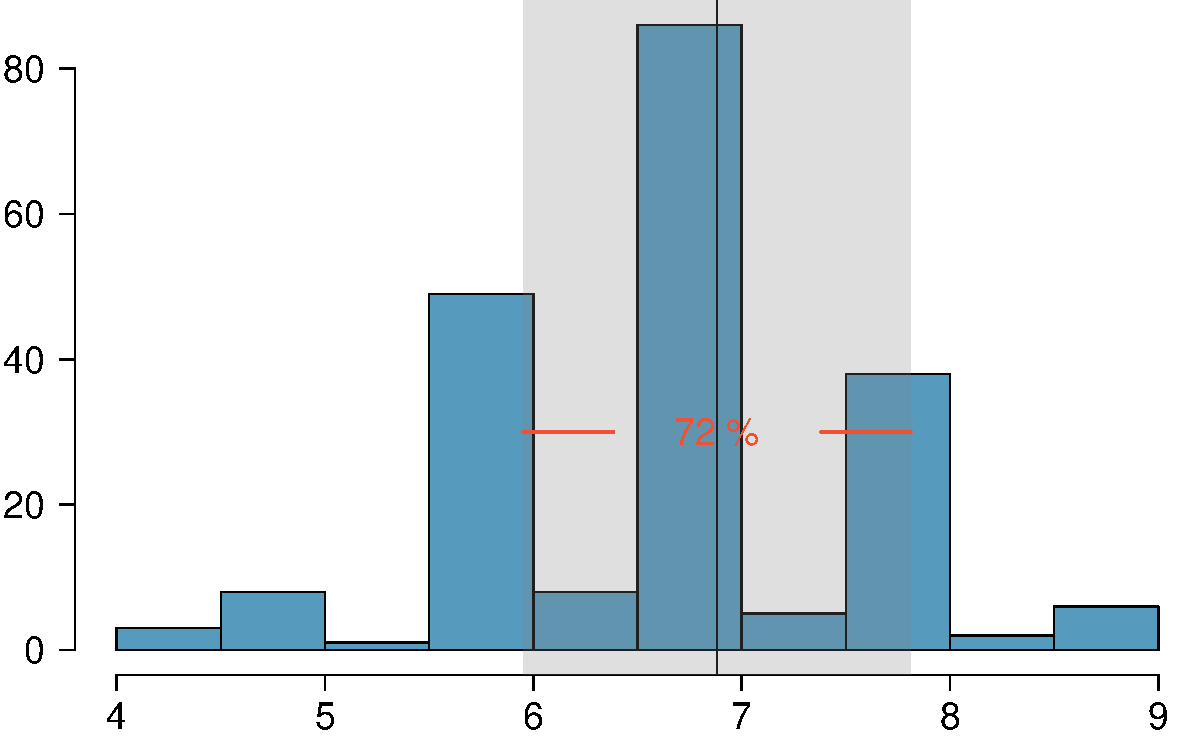
\includegraphics[width=0.75\textwidth]{4-1_normal_distribution/figures/sleep/sleep-hist-sd1} 
\end{center}
\vspace{-0.25cm}
\begin{itemize}
\item Mean = 6.88 hours, SD = 0.92 hrs
\item 72\% of the data are within 1 SD of the mean: $6.88 \pm 0.93$
\item[] \textcolor{white}{92\% of the data are within 2 SD of the mean: $6.88 \pm 2 \times 0.93$}
\item[] \textcolor{white}{99\% of the data are within 3 SD of the mean: $6.88 \pm 3 \times 0.93$}
\end{itemize}
}

\only<3 | handout:0>{
\begin{center}
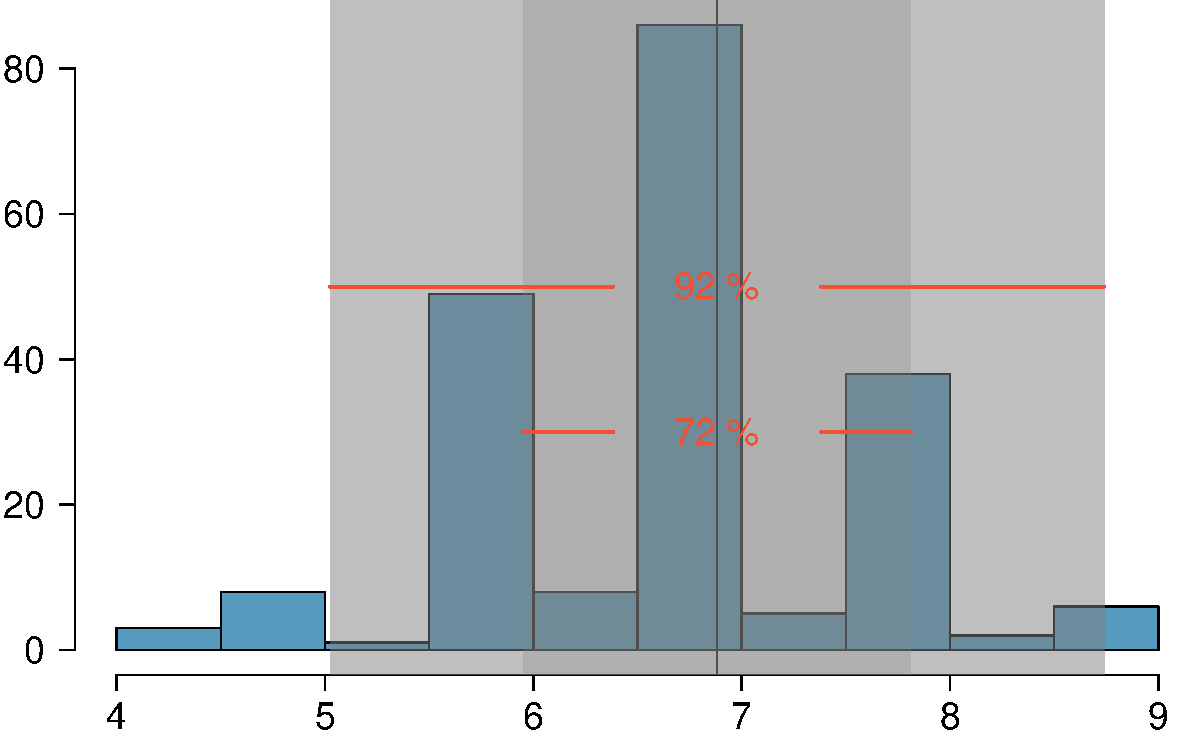
\includegraphics[width=0.75\textwidth]{4-1_normal_distribution/figures/sleep/sleep-hist-sd2} 
\end{center}
\vspace{-0.25cm}
\begin{itemize}
\item Mean = 6.88 hours, SD = 0.92 hrs
\item 72\% of the data are within 1 SD of the mean: $6.88 \pm 0.93$
\item 92\% of the data are within 1 SD of the mean: $6.88 \pm 2 \times 0.93$
\item[] \textcolor{white}{99\% of the data are within 3 SD of the mean: $6.88 \pm 3 \times 0.93$}
\end{itemize}
}

\only<4>{
\begin{center}
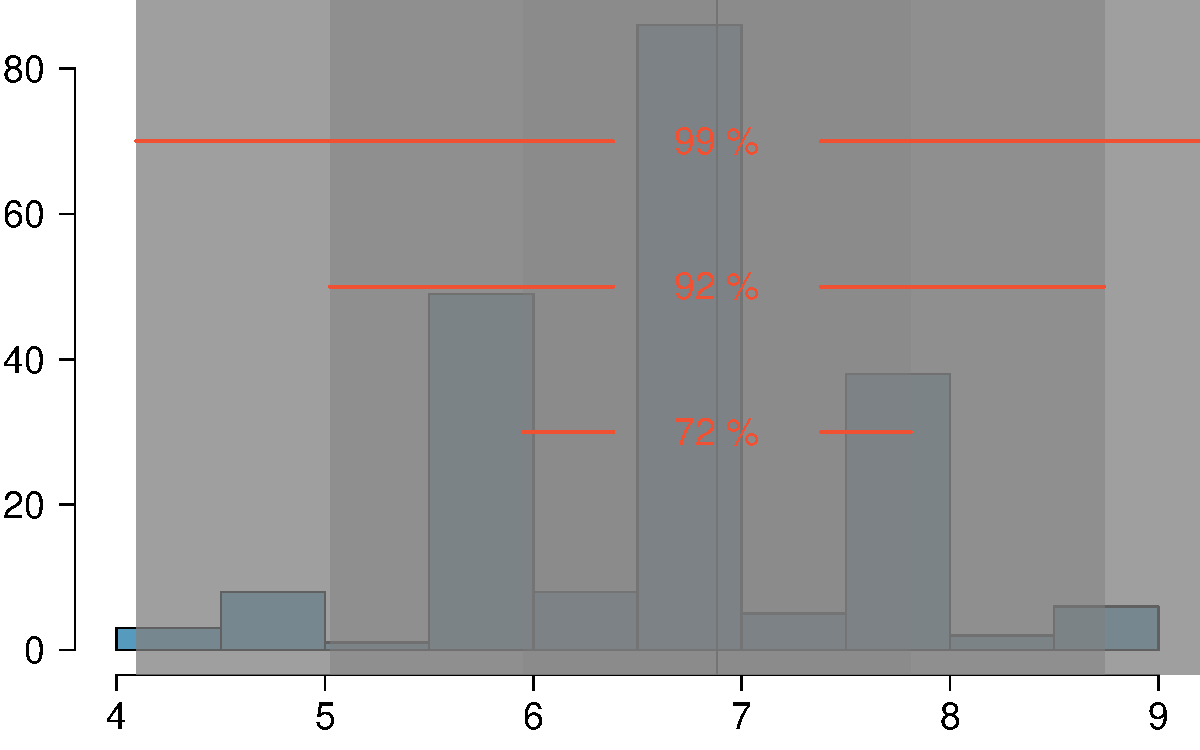
\includegraphics[width=0.75\textwidth]{4-1_normal_distribution/figures/sleep/sleep-hist-sd3} 
\end{center}
\vspace{-0.25cm}
\begin{itemize}
\item Mean = 6.88 hours, SD = 0.92 hrs
\item 72\% of the data are within 1 SD of the mean: $6.88 \pm 0.93$
\item 92\% of the data are within 2 SD of the mean: $6.88 \pm 2 \times 0.93$
\item 99\% of the data are within 3 SD of the mean: $6.88 \pm 3 \times 0.93$
\end{itemize}
}

\end{frame}

%%%%%%%%%%%%%%%%%%%%%%%%%%%%%%%%%%%%

\begin{frame}
\frametitle{Practice}

\pq{Which of the following is \underline{false}?}

\begin{enumerate}[(a)]
\item Majority of Z scores in a right skewed distribution are negative.
\solnMult{In skewed distributions the Z score of the mean might be different than 0.}
\item For a normal distribution, IQR is less than $2 \times SD$.
\item Z scores are helpful for determining how unusual a data point is compared to the rest of the data in the distribution.
\end{enumerate}

\end{frame}

%%%%%%%%%%%%%%%%%%%%%%%%%%%%%%%%%%%%


